\section{Assinatura de vídeo baseada em wavelets}

Esta abordagem foi escolhida por ter sido projetada especialmente para ser robusta a uma variedade de ataques fotométricos e de pós-produção, como modificações em contraste, brilho, contaminação por ruído e desfoque, inserção de logos, bordas e mudança de formato do quadro. Para se tornar ainda mais robustas a estes ataques, \citeauthor{Dutta2013} também descreve um fluxo de pré-processamento, abordado na Seção \ref{sec:preprocessamento}.

Após a etapa de pré-processamento e para ser usado como entrada para este algoritmo, os vídeos devem ser transformados para escala de cinza e ter suas intensidades normalizadas para o intervalo $[0,1]$. A assinatura proposta por \citeauthor{Dutta2013} é composta de uma parte baseada na transformada de Haar e em  outra baseda na distribuição espacial de gradientes.

\subsection{Transformada de Haar}

A transformada de Haar consiste em separar um sinal (ou quadro, neste caso) em 4 partes: 

\begin{itemize}
\item $LL$, que contém $1/4$ dos dados originais, removendo os detalhes.
\item $LH$, que contém a derivada na horizontal do quadro
\item $HL$, que contém a derivada na vertical do quadro
\item $HH$, que contém a derivada na diagonal do quadro
\end{itemize}

Ela pode ser aplicada de forma recursiva $n$ vezes, usando o quadro $I$ como entrada inicial do algoritmo e o $LL$ como entrada das chamadas subsequentes. Um exemplo do resultado da transformada de Haar pode ser visto na Figura ~\ref{figure:haar}.

\subsection{Assinatura baseada em wavelets}

\begin{enumerate}
\item Seja $I$ a imagem obtida após conversão para escala de cinza e normalização
% \item $F_i$ <- $F$
\item Para i de 1 até $n$, onde $n$ é o número de iterações da transformada de Haar
  \begin{enumerate}
    \item Aplicar a transformada de Haar sobre $I$ para obter um vetor com ($LL, LH, HL, HH$)
    \item Computar energia de $LH$, $HL$, $HH$ \footnote{$  \frac{1}{MN}\sum_{x=1}^M \sum_{y=1}^N |\mathbb{I}(x,y)|$}
  \end{enumerate}
\item Computar a energia da subimagem $I$, do último valor de $LL$ e concatenar estes valores em um vetor,

% \item Aplicar a transformada de Haar sobre a imagem $F$ com $n_w$ níveis de decomposição, o que irá resultar em quatro sub-bandas por decomposição. Estão são:
% 	\begin{enumerate}
% 	\item LL, versão reduzida da imagem $F_i$, tal que $i$ é a i-ésima decomposição
%     \item LH, detalhes da imagem resultados da aplicação de derivada discreta na horizontal
%     \item HL, detalhes da imagem resultados da aplicação de derivada discreta na vertical
%     \item HH, detalhes da imagem resultados da aplicação de derivada discreta na diagonal
% 	\end{enumerate}
% \item A cada nível, computar a energia de $LH$, $HL$, $HH$
% \item Computar a energia da subimagem $LL$ final
\item Concatenar os valores de energia obtidos nos passos anteriores para obter o descritor
\end{enumerate}

\begin{figure}[h]
  \centering
  \begin{tabular}{ccc}
  	\centering
<<<<<<< HEAD
    
\includegraphics[width=0.45\textwidth]{dados/figuras/ww.jpg} & \includegraphics[width=0.45\textwidth]{dados/figuras/ww_bw.jpg} \\ 
     a. Quadro original & b. Quadro em escala de cinza \\
    \multicolumn{2}{c}{\includegraphics[width=0.94\textwidth]{dados/figuras/ww_haar_.jpg}} \\
    \multicolumn{2}{c}{c. Após transformada de Haar}
  \end{tabular}
  \caption{Sequência de transformações feitas pelo algoritmo utilizando um quadro do filme Mulher Maravilha}
%   \includegraphics[width=0.8\textwidth]{dados/figuras/haar.png}
=======
    
\includegraphics[width=0.45\textwidth]{dados/figures/ww.jpg} & \includegraphics[width=0.45\textwidth]{dados/figures/ww_bw.jpg} \\ 
     a. Quadro original & b. Quadro em escala de cinza \\
    \multicolumn{2}{c}{\includegraphics[width=0.94\textwidth]{dados/figures/ww_haar_.jpg}} \\
    \multicolumn{2}{c}{c. Após transformada de Haar}
  \end{tabular}
  \caption{Sequência de transformações feitas pelo algoritmo utilizando um quadro do filme Mulher Maravilha}
%   \includegraphics[width=0.8\textwidth]{dados/figures/haar.png}
>>>>>>> 3e73fef3ea08fb1be8770ac872bddbc2ecfb216a
%   \caption{Resultado da Transformada de Haar. Os cantos superior direito, inferior esquerdo e inferior direito são, respectivamente, a derivada na horizontal(LH),derivada na vertical(HL) e derivada na diagonal(HH). O canto superior esquerdo é subdividido $N$ vezes em LH,HL e HH até o último nível em que não há mais divisão e que se chama LL}
  \label{figure:haar}
\end{figure}

\subsection{Assinatura baseada em distribuição espacial de gradientes}

\begin{enumerate}
\item Dado um quadro $I$ já pré-processado, aplicar a transformada de Haar com um nível e obter um vetor com $LL,LH,HL,HH$
\item Computar o gradiente de $LL$\footnote{A imagem LL é usada pois contém menos ruído que a imagem original graças à transformada de Haar}
\item Dividir a imagem de gradiente em $N_p$ partições com o mesmo tamanho
\item Para cada partição, computar um histograma de gradiente
\item Concatenar os histogramas  para obter o descritor
\end{enumerate}